\chapter{First hitting time boost}
In this chapter, we propose a component-wise boosting algorithm for fitting the inverse gaussian first hitting time model to survival data.

\section{Simulation of survival data}
We wish to simulate survival times $\ti,i=1,\ldots,N$ with censoring. We first draw survival times $\tilde{t}_i$ from some survival time distribution $f(\cdot)$. If this distribution has a closed form probability distribution function, we can draw from it directly. If not, we might use some an inverse sampling method, e.g. by drawing unit exponentials and using a corresponding transformation.

To censor the data, we draw censoring times $W_i\sim f(\cdot),i=1,\ldots,N$, from a more right-tailed distribution, meaning we want to get many, but not all, $W_i$'s to be larger than the $\tilde{t}_i$'s. We let the observed survival times then be $t_i=\min(\tilde{t}_i,W_i)$.
The corresponding observed indicator, $\di$, is then set equal to 1 if the actual survival time was observed, i.e., if $\ti<W_i$. We end up with a set of $N$ tuples $(t_i,\delta_i),i=1,\ldots,N$. Note that this scheme incorporates independent censoring: The censoring time is independent of the survival times. This does not pose a problem. Summary of the procedure:

\begin{algorithm}
\caption{Generating survival data from Inverse Gaussian distribution}
\label{algo:FHT-sim}
\begin{enumerate}
    \item Given design matrices $\X$, $\Z$ and true parameter vectors $\bbeta$ and $\bgamma$.
    \item Link covariates and parameters using link functions
        \begin{align*}
            \ln y_0&=\bbeta^T\X \\
            \mu&=\bgamma^T\Z.
        \end{align*}
    \item Draw $N$ survival times $(t_i)_{i=1}^N$ from IG$(\mu,y_0)$.
    \item Draw a censoring time $W$ from some distribution which is independent of the data.
    \item Right censor data by choosing $\widetilde{t}_i=\min(t_i,W)$. The indicator on whether observation $i$ was observed or not is then $\delta_i=I(\widetilde{t}_i=t_i)$.
    \item The simulated data set is $(t_i,\delta_i)$.
\end{enumerate}
\end{algorithm}


\section{Algorithm}
We apply the component-wise boosting algorithm \ref{algo:fhtboost} with loss function $\rho(\mu,\y0)=-\log\loss{y_0,\mu}$. We differentiate the loss function with respect to these two and get .... For more details on the derivation, see \ref{appendix}. \todo{Maybe use $b$ instead of $y_0$, to not get subscript chaos?}

\begin{algorithm}
\caption{FHT Boost with twodimensional loss function}
\label{algo:fhtboost}
\begin{enumerate}
    \item Initialize the $n$-dimensional vectors $\hat{y}_0^{[0]},\hat{\mu}^{[0]}$, with offset values, e.g. with $\hat{y}_0^{[0]}=\0,\ldots,\hat{\mu}^{[0]}=\0$. Alternatively, one can use the maximum likelihood estimates as offset values.
    \item For both components of the loss function, specify base learners, in particular, a component-wise base learner which can be used for each of the $p$ variables used in $\X$ corresponding to $y_0$ and the $d$ variables in $\Z$ corresponding to $\mu$. Like earlier, the base learner takes one input variable and has one output variable. Examples include least squares linear regression.
    \item Set $m=0$ and $\nu=0.1$.
    \item Increase $m$ by 1.
    \begin{enumerate}
        \item If $m>m_{\text{stop},y_0}$, proceed to step 4 e). If not, compute the negative partial derivative $-\frac{\partial\rho}{\partial y_0}$ and evaluate at $\hat{f}^{[m-1]}(X_i,Z_i)=\left(\hat{y}_0^{[m-1]}(X_i),\hat{\mu}^{[m-1]}(Z_i)\right)_{i=1,\ldots,n}$. This yields the negative gradient vector $U_{y_0}^{[m-1]}=\left(U_{i,y_0}^{[m-1]}\right)_{i=1,\ldots,n}:=\left(-\frac{\partial}{\partial y_0}\rho\left(Y_i,\hat{f}^{[m-1]}(X_i,Z_i)\right)\right)_{i=1,\ldots,n}$.
        \item Fit the negative gradient vector $U_{y_0}^{[m-1]}$ to each of the $p$ components of $\X$ separately (i.e. to each predictor variable) using the base learners specified in step 2. This yields $p$ vectors of predicted values, where each vector is an estimate of the negative gradient vector $U_{y_0}^{[m-1]}$.
        \item Select the component of $\X$ which best fits $U_{y_0}{[m-1]}$ according to $R^2$. Set $\hat{U}_{y_0}^{[m-1]}$ equal to the fitted values of the corresponding best model fitted in the previous step.
        \item Update $\hat{y}_0^{[m-1]}\gets\hat{y}_0^{[m-1]}+\nu\hat{U}_{y_0}^{[m-1]}$.
        \item If $m>m_{\text{stop},\mu}$, proceed to step 4 j). If not, compute the negative partial derivative $-\frac{\partial\rho}{\partial \mu}$ and evaluate at $\hat{f}^{[m-1]}(X_i,Z_i)=\left(\hat{y}_0^{[m-1]}(X_i),\hat{\mu}^{[m-1]}(Z_i)\right)_{i=1,\ldots,n}$. This yields the negative gradient vector $U_{\mu}^{[m-1]}=\left(U_{i,\mu}^{[m-1]}\right)_{i=1,\ldots,n}:=\left(-\frac{\partial}{\partial \mu}\rho\left(Y_i,\hat{f}^{[m-1]}(X_i,Z_i)\right)\right)_{i=1,\ldots,n}$.
        \item Fit the negative gradient vector $U_{\mu}^{[m-1]}$ to each of the $p$ components of $\Z$ separately (i.e. to each predictor variable) using the base learners specified in step 2. This yields $d$ vectors of predicted values, where each vector is an estimate of the negative gradient vector $U_{\mu}^{[m-1]}$.
        \item Select the component of $\Z$ which best fits $U_{\mu}{[m-1]}$ according to $R^2$. Set $\hat{U}_{\mu}^{[m-1]}$ equal to the fitted values of the corresponding best model fitted in the previous step.
        \item Update $\hat{\mu}^{[m-1]}\gets\hat{\mu}^{[m-1]}+\nu\hat{U}_{\mu}^{[m-1]}$.
        \item Update $\hat{f}^{[m]}\gets\hat{f}^{[m-1]}$.
        \item If $m>\max(m_{\text{stop},y_0},m_{\text{stop},\mu})$, go to step 5. If not, repeat step 4.
    \end{enumerate}
    \item Return $\hat{f}^{[m]}$.
\end{enumerate}
\end{algorithm}
We might call this cyclical boosting.

\subsection{Boost in same}
Another way to do this is to only boost one component in each iteration. The component might be corresponding to $X$, or it might be corresponding to $Z$.


% First tried cyclical boosting.
% Then tried non-cyclical, with comparing RSS. Doesn't work; not on the same scale.
% Then tried using non-cyclical, comparing instead the loss function instead of rss.


\section{Simulation experiments}
In this section, I will discuss how I tried validating the boosting method I have developed. To see if the method works, we must see if 1) it converges to the maximum likelihood estimates, and 2) if it does so in a high-dimensional setting as well.

\subsection{Small example}
Let parameter vectors be two dense $\bbeta=(2,0.1,0.2)$ and $\bgamma=(-1, -0.1, 0.1)$. Let $X$ and $Z$ be such and such, drawn from a beta distribution.
We simulate data using Algorithm \ref{algo:FHT-sim}, with the censoring time $W$ being drawn from a distribution $\exp(0.1)$. The resulting survival times have the following Kaplan-Meier plot.
\begin{figure}[H]\centering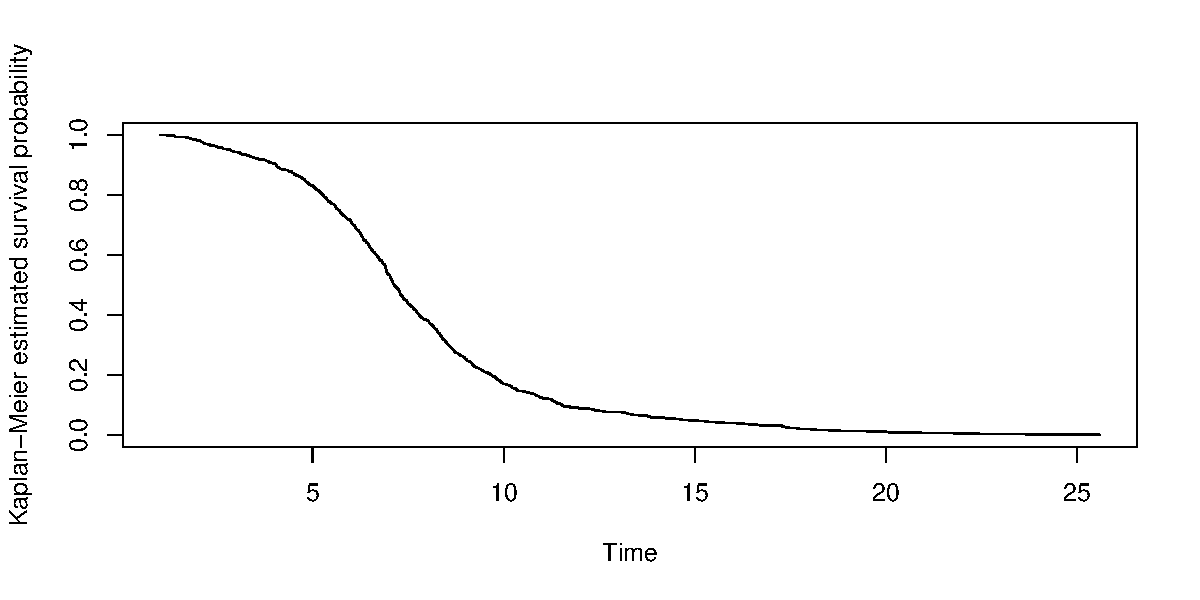
\includegraphics[scale=0.4]{figures/case1.pdf}\end{figure}

\subsection{Large example with uncorrelated matrices}
Here, $N$ is 1000. We let $\bbeta$ be a large vector of size $p=10001$, and $\bgamma$ be a small vector of size $d=16$. We imagine $X$, corresponding to $\bbeta$, be gene expressions, whereas $Z$, corresponding to $\bgamma$ be clinical measurements. Specifically, we set the intercept term in $\bbeta$ to be 2.0, and the first 35 elements to be 0.1. We set the rest to be 0. For $\bgamma$, we set the intercept term to be -1, and in similar fashion, let the first 5 elements have a non-zero value of -0.1. Here also we set the remaining 10 elements to be 0.
We also here draw $X$ and $Z$ from a beta distribution. The resulting survival times have the following Kaplan-Meier plot.
\begin{figure}[H]\centering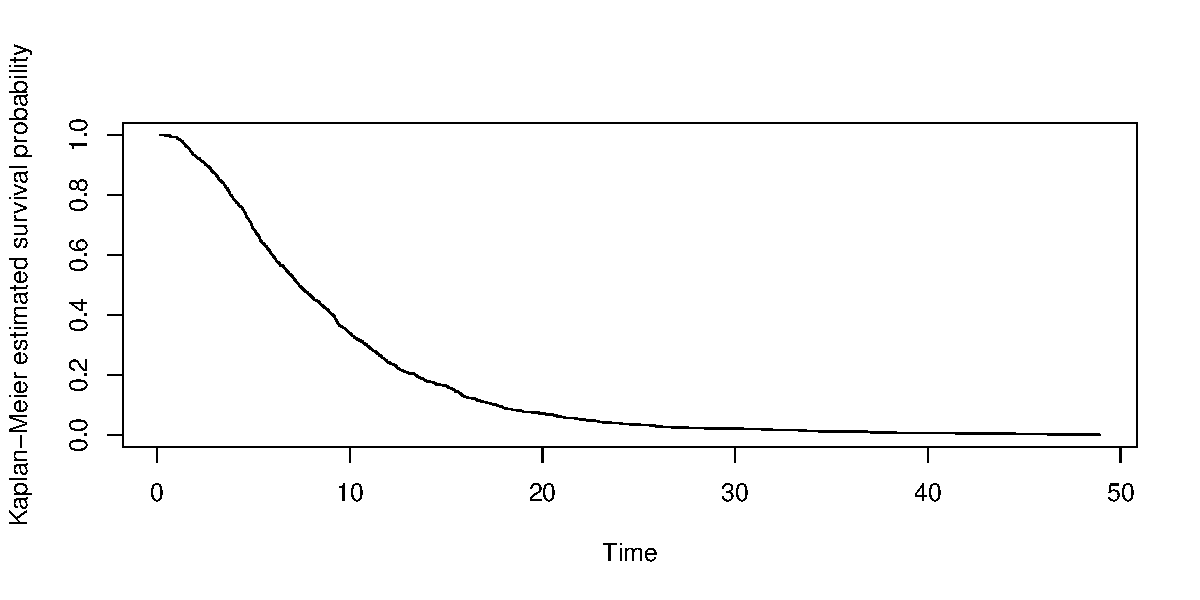
\includegraphics[scale=0.4]{figures/case2.pdf}\end{figure}

\subsection{Large example with correlated matrices}
Here, $N$ is 1000. We let $\bbeta$ be a large vector of size $p=10001$, and $\bgamma$ be a small vector of size $d=16$. We imagine $X$, corresponding to $\bbeta$, be gene expressions, whereas $Z$, corresponding to $\bgamma$ be clinical measurements. Specifically, we set the intercept term in $\bbeta$ to be 2.0, and the first 35 elements to be 0.1. We set the rest to be 0. For $\bgamma$, we set the intercept term to be -1, and in similar fashion, let the first 5 elements have a non-zero value of -0.1. Here also we set the remaining 10 elements to be 0.
